\begin{mainquestion}{diodepullup}{Diode-Connected Transistor as Pull-Up Resistor}

A diode-connected transistor is used as a replacement for the pull-up resistor in a common source (CS) amplifier.

\begin{center}
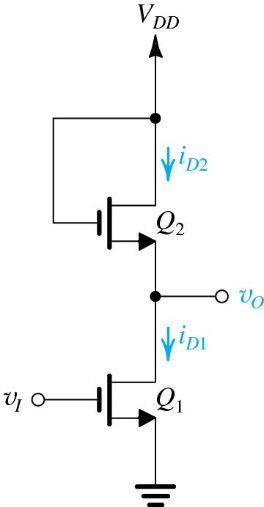
\includegraphics[width=2in]{image16.jpeg}
\end{center}

\begin{partquestion}{saturationrange}{Determine the range of $v_{I}$ over which $Q_{1}$ is in saturation.}
\begin{answer}
$Q_{1}$ will be in saturation as long as $v_{I} = V_{GS} > V_{t}$ and $v_{O} > v_{I} - V_{t}$, so we have the constraint:

\[
V_{t} < v_{I} < v_{O} + V_{t}.
\]
\end{answer}
\end{partquestion}

\begin{partquestion}{deriveoutput}{Show that for this range the output voltage is:

\[
v_{O} = V_{DD} - V_{t} + \sqrt{\frac{\left(W / L\right)_{1}}{\left(W / L\right)_{2}}} V_{t} - \sqrt{\frac{\left(W / L\right)_{1}}{\left(W / L\right)_{2}}} v_{I}
\]

assuming that both transistors have the same threshold voltages $V_{t}$. Thus, the circuit functions as a linear amplifier even for large input signals.}
\begin{answer}
We know from the previous homework that $Q_{2}$ will be in saturation as long as it is not cutoff, and $i_{D1} = i_{D2}$. So we can equate the expressions for $Q_{1}$ and $Q_{2}$ current in saturation:

\begin{align*}
    \frac{1}{2} k' \left(\frac{W}{L}\right)_1(V_{GS1} - V_t)^2 &= \frac{1}{2} k' \left(\frac{W}{L}\right)_2(V_{GS2} - V_t)^2\\
    \left(\frac{W}{L}\right)_1(V_I - V_t)^2 &= \left(\frac{W}{L}\right)_2(V_{DD} - v_O - V_t)^2\\
    \sqrt{\left(\frac{W}{L}\right)_1}(V_I - V_t) &= \sqrt{\left(\frac{W}{L}\right)_2}(V_{DD} - v_O - V_t)\\
    \sqrt{\frac{(W / L)_1}{(W / L)_2}}(V_I - V_t) &= V_{DD} - v_O - V_t\\
    v_O &= V_{DD} - V_t - \sqrt{\frac{(W / L)_1}{(W / L)_2}}(V_I - V_t)\\
    v_{O} &= V_{DD} - V_{t} + \sqrt{\frac{\left(W / L\right)_{1}}{\left(W / L\right)_{2}}} V_{t} - \sqrt{\frac{\left(W / L\right)_{1}}{\left(W / L\right)_{2}}} v_{I}
\end{align*}
\end{answer}
\end{partquestion}

\begin{partquestion}{gaincalc}{Find the voltage gain for $W_{1} = 10\ \mu\text{m}$, $W_{2} = 0.8\ \mu\text{m}$ and $L_{1} = L_{2} = 0.18\ \mu\text{m}$. Given that $L$ is often constrained for a given technology, describe a potential approach to increasing the gain for this amplifier configuration.}
\begin{answer}
The voltage gain is the slope (at the operating point) on the transfer curve of $v_{O}$ vs. $v_{I}$. From the result in (b), we can calculate:

\begin{align*}
    A_v &= \frac{d v_o}{d v_I} \\
    &= - \sqrt{\frac{(W / L)_1}{(W / L)_2}} \\
    &= - \sqrt{\frac{10/0.18}{0.8/0.18}} \\
    &= - \sqrt{\frac{10}{0.8}} \\
    &= - 3.54
\end{align*}

The simplest way to adjust the gain is by controlling the transistor widths. By making the bottom transistor wider (which is generally easier than making a relatively narrow one narrower!), we can easily increase the gain.
\end{answer}
\end{partquestion}

\end{mainquestion}
